\documentclass{article}

%%%%%%%%%%%%%%%%%%%%%%%%%%%%%%%%
% PACKAGES
%%%%%%%%%%%%%%%%%%%%%%%%%%%%%%%%
\usepackage{times}
\usepackage{fullpage}
\usepackage{latexsym}
\usepackage{amsmath}
\usepackage{amssymb}
\usepackage{mathtools}
\usepackage{accents}
\usepackage{tikz}
\usepackage{pgfplots}
\usepackage[ruled]{algorithm}
\usepackage{algpseudocode}
\usepackage{dsfont}
\usepackage[bf]{caption}
\usepackage{hyperref}
\hypersetup{
    bookmarks=true,         % show bookmarks bar?
    unicode=false,          % non-Latin characters in AcrobatÕs bookmarks
    pdftoolbar=true,        % show AcrobatÕs toolbar?
    pdfmenubar=true,        % show AcrobatÕs menu?
    pdffitwindow=false,     % window fit to page when opened
    pdfstartview={FitH},    % fits the width of the page to the window
    pdftitle={My title},    % title
    pdfauthor={Author},     % author
    pdfsubject={Subject},   % subject of the document
    pdfcreator={Creator},   % creator of the document
    pdfproducer={Producer}, % producer of the document
    pdfkeywords={keyword1} {key2} {key3}, % list of keywords
    pdfnewwindow=true,      % links in new window
    colorlinks=true,       % false: boxed links; true: colored links
    linkcolor=red,          % color of internal links (change box color with linkbordercolor)
    citecolor=blue,        % color of links to bibliography
    filecolor=magenta,      % color of file links
    urlcolor=cyan           % color of external links
}
\usepackage{amsthm}
\usepackage{natbib}
\usepackage[capitalize]{cleveref}
\usepackage{graphicx}
\usepackage{parskip}
%%%%%%%%%%%%%%%%%%%%%%%%%%%%%%%%
% MACROS
%%%%%%%%%%%%%%%%%%%%%%%%%%%%%%%%
\newcommand{\defined}{\vcentcolon =}
\newcommand{\rdefined}{=\vcentcolon}
\newcommand{\E}{\mathbb E}
\newcommand{\Var}{\operatorname{Var}}
\newcommand{\calF}{\mathcal F}
\newcommand{\sr}[1]{\stackrel{#1}}
\newcommand{\set}[1]{\left\{#1\right\}}
\newcommand{\ind}[1]{\mathds{1}\!\!\set{#1}}
\newcommand{\argmax}{\operatornamewithlimits{arg\,max}}
\newcommand{\argmin}{\operatornamewithlimits{arg\,min}}
\newcommand{\floor}[1]{\left \lfloor {#1} \right\rfloor}
\newcommand{\ceil}[1]{\left \lceil {#1} \right\rceil}
\newcommand{\eqn}[1]{\begin{align}#1\end{align}}
\newcommand{\eq}[1]{\begin{align*}#1\end{align*}}
\newcommand{\Ber}{\operatorname{Bernoulli}}
\renewcommand{\P}[1]{\operatorname{P}\left\{#1\right\}}


%%%%%%%%%%%%%%%%%%%%%%%%%%%%%%%%
% THEOREMS
%%%%%%%%%%%%%%%%%%%%%%%%%%%%%%%%
\theoremstyle{plain}
\newtheorem{theorem}{Theorem}
\newtheorem{proposition}[theorem]{Proposition}
\newtheorem{lemma}[theorem]{Lemma}
\newtheorem{corollary}[theorem]{Corollary}
\theoremstyle{definition}
\newtheorem{definition}[theorem]{Definition}
\newtheorem{assumption}[theorem]{Assumption}
\newtheorem{remark}[theorem]{Remark}
\newtheorem{example}[theorem]{Example}

\title{Intervention Bandits}
\author{Blah blah}

\begin{document}
\def\ci{\perp\!\!\!\perp}
\maketitle

\begin{abstract}
An abstract.
\end{abstract}

\section{Introduction}

Useful references are: \cite{BC12}.

\section{Notation}

Assume we have a known causal model with binary variables $\boldsymbol{X} = \{X_{1}..X_{K}\}$ that independently cause a target variable of interest $Y$. We can run sequential experiments on the system, where at each timestep $t$ we can select a variable on which to intervene and then we observe the complete result, $(\boldsymbol{X}_{t},Y_{t})$ This problem can be viewed as a variant of the multi-armed bandit problem.


Let $p \in [0,1]^K$ be a fixed and known vector. In each time-step $t$:
 
\begin{enumerate}
\item The learner chooses an $I_t \in \set{1,\ldots, K}$ and $J_t \in \set{0,1}$.
\item Then $X_t \in \set{0,1}^K$ is sampled from a product of Bernoulli distributions, $X_{t,i} \sim \Ber(p_i)$ 
\item The learner observes $\tilde X_t \in \set{0,1}^K$, which is defined by 
\eq{
\tilde X_{t,i} = \begin{cases}
X_{t,i} &\text{if } i \neq I_t \\
J_t & \text{otherwise}\,.
\end{cases}
}
\item The learner receives reward $Y_t \sim \Ber(q(\tilde X))$ where $q:\set{0,1}^K \to [0,1]$ is unknown and arbitrary.
\end{enumerate}
The expected reward of taking action $i,j$ is $\mu_{i,j} = \E[q(X)|do(X_i = j)]$. The optimal reward and action are $\mu^*$ and $(i^*,j^*)$ respectively,
where $(i^*,j^*) = \argmax_{i,j} \mu_{i,j}$ and $\mu^* = \mu(i^*,j^*)$. The $n$-step cumulative expected regret is
\eq{
R_n = \E \sum_{t=1}^n \left(\mu^* - \mu_{I_t,J_t}\right).
}

\section{Estimating $\mu_{i,j}$}
The most natural way to estimate $\mu_{i,j}$ is to compute an empirical estimate based on samples when that action was taken. This approach would
lead directly to the UCB algorithm with $2K$ actions and a regret bound that depended linearly on $K$. 

In this instance we can significantly
outperform the standard approach by exploiting the known causal structure of the problem.

\eq {
P(Y|do(X_i=j)) &= P(Y|X_i = j)\\
 &= \sum_{b}P(Y|X_i = j,X_a = b)P(X_a = b|X_i = j) \\
 &= \sum_{b}P(Y|X_i = j,X_a = b)P(X_a = b), \; \forall \, a \in \{1...K\}/i \text{ as } X_a \ci X_i\\
 &= \sum_{b}P(Y|X_i = j,do(X_a = b))P(X_a = b) 
}


\subsection{Estimators}
\label{sec:estimators}
Fix some time-step $t$ and $i \in \set{1,\ldots,K}$ and $j \in \set{0,1}$. 

Let $\hat{\mu}_a$ be an empirical estimator for $P(Y|do(X_i=j))$ obtained via marginalization over $X_a$.

\eq {
\hat{\mu}_a &=
\begin{cases}
\frac{m_{a,1}}{n_{a,1}}p_a+\frac{m_{a,0}}{n_{a,0}}(1-p_a) & \text{if } a \neq{i} \\
\frac{m_{i,j}}{n_{i,j}} & \text{if } a=i \\
\end{cases}\\
\text{where:}\\
m_{a,b}    &= \sum_{s=1}^t \ind{X_i = j, I = a,J = b, Y = 1}_s \\
n_{a,b}    &= \sum_{s=1}^t \ind{X_i = j, I = a,J = b}_s \\
}



This gives $K$ estimators $\{\hat{\mu_1}...\hat{\mu_K}\}$ to be pooled into a single estimator $\hat{\mu}$.

\eq {
\hat{\mu} &= \sum^{K}_{a=1}w_a\hat{\mu}_a=w_i \frac{m_{i,j}}{n_{i,j}}+ \sum_{a \neq i} w_a \left[p_a \frac{m_{a,1}}{n_{a,1}} + (1 - p_a) \frac{m_{a,0}}{n_{a,0}}\right]\\
}



If $p$ is not known, these expression are unchanged except that $p_a$ is replaced with $\hat{p}_a$

\eq{
\hat{p}_a = \frac{\sum_{s=1}^{t} \ind{X_a=1,I \neq a}_s}{\sum_{s=1}^{t} \ind{I \neq a}_s}
}
\subsection{Observe then exploit}

Basic idea - observe until the uncertainty on all actions is smaller than $\epsilon$, then exploit (or switch to standard UCB). This is only really going to work if $p_a \sim 0.5$. 

Bounds on regret: when observing the regret for each timestep is at most 1 (since the reward is $\in [0,1]$). When exploiting regret it at most $\epsilon$. If the horizon is $n$, the cost of exploiting $< \epsilon n$ and the cost of observing is $O(1/\epsilon^2)$ (this comes from how quickly we converge to within $\epsilon$ for all arms). 

\eqn{
R_n = O(n\epsilon+\frac{1}{\epsilon^2})
}

Differentiating and selecting $\epsilon = (\frac{2}{n})^{1/3}$ to minimize the regret yields:

\eqn{
R_n = O(n^{2/3})
}

For each arm $X_i = j$, we have:

\eqn{
\hat{\mu}_{ij} = \frac{m_{ij}}{n_{ij}}
}

where

\eqn{
m_{i,j}    &= \sum_{s=1}^t \ind{X_i = j, Y = 1} \\
n_{i,j}    &= \sum_{s=1}^t \ind{X_i = j} \\
}

and Hoeffding's Inequality gives:

\eqn {
P\left(|\hat{\mu}_{ij} - \mu_{ij}| > \sqrt{\frac{1}{2n_{ij}}\log{\frac{2}{\delta}}}\right) \leq \delta
}

\section{Observe until number of plausibly optional arms $< \alpha$}

Define the set of plausibly optimal arms to be those with an upper confidence bound that is higher than the largest lower confidence bound.

\eqn {
A_t = \{k : UB(k) \geq max_{k'}(LB(k'))  \}
}

We then observe until the size of this set is less than some value $\alpha$ before switching to UCB. This takes into account that we don't need narrow confidence bounds on the arms with very low expected reward. Once we start doing UCB, we keep track of the ucb bound separately and for each arm use whichever bounds are narrower. 

\subsection{Regret during observe phase}

Let $n$ be the number of timesteps until the size of the set $A_t$ falls below $\alpha$ or we reach the overall horizon $T$

\eqn {
n = \min(\{t:size(A_t)< \alpha, T\})
}

Let $Q(k)$ be the expected reward for arm $k$ and $\mu^*$ be the expected reward for the best arm.

\eqn {
R_n = & \max_{i=1...K} E\left[\sum_{t=1}^n Y_{it} - \sum_{t=1}^n Y_{I_t,t} \right] \\
= & E[n]\left(\mu^*  - E[Q]\right) 
}

Without loss of generality, assume the arms are ordered from best to worst.

\eqn{
& Q(k = 1...K) = [\mu^*, \mu^*-d_2 ... \mu^*-d_k] \\
&\implies E[Q] = \mu^* - \frac{1}{K}\sum_{k=2}^K d_k \\
&\implies  R_n = E[n]\left(\frac{1}{K}\sum_{k=2}^K d_k \right)
}

Whenever the following two statements hold only arms with indexes less than $\alpha$ can be in the set $A_t$:

\eqn {
& \mu^* - \hat{\mu}^* \leq \frac{d_\alpha}{2} \\
& \hat{\mu_k} - \mu_k \leq \frac{d_k}{2} \; \forall k \geq \alpha 
}

\eqn{
\label{eq:proboverlap}
\implies \rho(t) \equiv P(\exists k \in A_t: k \geq \alpha)  \leq P(\mu^* - \hat{\mu}^* > \frac{d_\alpha}{2}) + \sum_{k=\alpha}^K P( \hat{\mu_k} - \mu_k > \frac{d_k}{2})
}


\eqn {
P(n > t) = \begin{cases} 0 & \text{if } t \geq T \\
P(\exists k \in A_t: k \geq \alpha) & \text{otherwise}
\end{cases}
}


We now concentrate bounding \ref{eq:proboverlap}. For random variables $W_{sij} = P(Y|X_i=j)$ drawn from a Bernoulli distribution with mean $p_{ij}$ the Chernoff inequality gives:

\eqn {
& P(\frac{1}{t}\sum_s W_{sij} - p_{ij} \geq \gamma) \leq \exp(-\frac{t\gamma^2}{2p_{ij}(1-p_{ij})+2\gamma/3}) \\
\implies & P(\frac{1}{t}\sum_s \frac{W_{sij}}{p} - \frac{p_{ij}}{p} \geq \epsilon) = P(\hat{\mu}_k - \mu_k \geq \epsilon) \leq \exp(-\frac{tp\epsilon^2}{2+2\epsilon/3}) = \exp(-\frac{t\epsilon^2}{4+4\epsilon/3})
}
Where $p_{ij} = P(Y = 1, X_i = j) \leq P(X_i=j) = p = 1/2 \;\;\; \forall(i,j)$

Similarly, 
\eqn {
P(\mu^* - \hat{\mu}^* \geq \epsilon) \leq exp(-tp^2\epsilon^2) = exp(-\frac{t\epsilon^2}{4})
}

\eqn {
\implies \rho(t) \leq \exp(-\frac{ d_\alpha^2 t}{16}) + \sum_{k=\alpha}^K exp(-\frac{d_k^2 t}{16(1+d_k/6)})
}


\eqn{ 
E[n] = & \sum_{t=1}^T P(n \geq t) \leq \sum_{t=1}^T \rho(t) \\
= & \min \left(T, \frac{1 - e^{-d_\alpha^2 T/16}}{e^{d_\alpha^2 /16} -1 } +  \sum_{k=\alpha}^K \frac{1 - e^{-d_k^2 T/16(1+d_k/6)}}{e^{d_k^2 /16(1+d_k/6)} -1 } \right)
}

Since the regret is $R_n = E[n]\left(\frac{1}{K}\sum_{k=2}^K d_k \right)$ the worst case is that just enough of the differences $d_k$ are $0$ to make $E[n] = T$ and the remainder are $1$. This occurs if $d_\alpha = 0$, In this case the regret is:

\eqn {
R_n = T \left(\frac{K-(\alpha+1)}{K}\right)
}








\subsection{Bounding a weighted sum of unbiased estimators with McDiarmid's Ineqaulity}

McDiarmid's Inequality states:
If $X_i \ci X_j$ and 
\eqn{
|\phi(X_1...X_i...X_N) - \phi(X_1...X_i^{'}...X_N)| < c_i \;\; \forall i
}
\eqn{
& P\left(|\phi(\boldsymbol{X}) - E[\phi(\boldsymbol{X})]| \geq \epsilon \right) \leq 2 \exp \left(-\frac{2 \epsilon^2}{\sum_{i}c_i^2} \right)\\
\label{eqn:McDiarmid}
& P\left(|\phi(\boldsymbol{X}) - E[\phi(\boldsymbol{X})]| \geq 
\sqrt{\frac{\sum_{i}c_i^2}{2}\log{\frac{2}{\delta}}} 
\right) \leq \delta
}


In our problem, for each variable $V_i$ and value $j$ we have:

\eqn{
\hat{\mu}_a = \tilde{P}(Y|V_i = j)= \begin{cases}
\frac{p_a}{n_{a1}}\sum_{s=1}^{n_{a1}}X_{a1,s} + \frac{1-p_a}{n_{a0}}\sum_{s=1}^{n_{a0}}X_{a0,s} & \text{ if $a \neq i$}\\
\sum_{s=1}^{n_i}X_s & \text{if $a = i$}
\end{cases}
}

where $X_{a1,s}  \sim P(Y|V_i = j, do(V_a = 1))$ and $X_{a0,s}  \sim P(Y|V_i = j, do(V_a = 0))$, both $\in [0,1]$. We then pool $\{\hat{\mu}_1 ... \hat{\mu}_K \}$ to get a single estimate.

\eqn {
\hat{\mu} = \tilde{P}(Y|V_i = j)= \sum_a w_a \hat{\mu}_a \text{, where } \sum_a w_a = 1
}

Let 

\eqn {
\hat{\mu} = \phi(\boldsymbol{X}) = \sum_{a \neq i} w_a \left[ 
\frac{p_a}{n_{a1}}\sum_{s=1}^{n_{a1}}X_{a1,s} + \frac{1-p_a}{n_{a0}}\sum_{s=1}^{n_{a0}}X_{a0,s}
\right] + \frac{w_i}{n_i} \sum_{s=1}^{n_i}X_{i,s}
}

Note: this treats the number of samples $n_i$,$n_{a1}$, and $n_{a0}$ as fixed. Even for fixed actions, the latter two are still random variables that depend on $\boldsymbol{p}$  Will this bound still hold?  



\eqn {
&\phi(...X_{\alpha 1,s}...) - \phi(...X_{\alpha 1,s}^{'}...) \leq w_\alpha \frac{p_\alpha}{n_{\alpha 1}} \\
&\phi(...X_{\alpha 0,s}...) - \phi(...X_{\alpha 0,s}^{'}...) \leq w_\alpha \frac{1-p_\alpha}{n_{\alpha 0}}\\
& \phi(...X_i...) - \phi(...X_i^{'}...) \leq \frac{w_i}{n_i}
}


\eqn{
\sum_i c_i^2 = & n_i \left(\frac{w_i}{n_i}\right)^2+ \sum_a \left[ n_{a1}\left(w_a \frac{p_a}{n_{a1}}\right)^2 + n_{a0}\left(w_a \frac{1-p_a}{n_{a0}}\right)^2\right]\\
= & \frac{w_i^2}{n_i}+ \sum_a w_a^2 \left(\frac{p_a^2}{n_{a1}}+  \frac{(1-p_a)^2}{n_{a0}} \right) \\
\label{eq:tominimize}
= & \sum_a w_a^2 f(a) \text{, where }\\ 
f(a) =& \begin{cases}
\frac{p_a^2}{n_{a1}}+  \frac{(1-p_a)^2}{n_{a0}}  & a \neq i\\
\frac{1}{n_i} & a = i
\end{cases}
}

We want to choose weights $\boldsymbol{w}$ so as to minimize \ref{eq:tominimize} subject to the constraint $\sum_a w_a = 1$.


The minimum (assuming it exists) should occur at a critical point of:

\eqn {
L(w_1...w_k,\lambda) = \sum_a w_a^2 f(a) + \lambda((\sum_a w_a)-1)
}

\eqn{
& \frac{\partial L}{\partial w_a}  = 2 w_a f(a) + \lambda = 0 \\
& \implies w_a =  \frac{-\lambda}{2 f(a)}\\
& \frac{\partial L}{\partial \lambda}  = (\sum_a w_a)-1= 0 \\
& \implies -\frac{\lambda}{2}\sum_a \frac{1}{f(a)} = 1
 \implies \lambda = -\frac{2}{\sum_a \frac{1}{f(a)}}\\
& \implies w_a = \frac{1}{f(a)\sum_a \frac{1}{f(a)}} \\
\label{eqn:sumofsquares}
& \implies \sum_i c_i^2 = \frac{1}{\sum_a \frac{1}{f(a)}} 
}

Substituting \ref{eqn:sumofsquares} into the McDiarmid inequality \ref{eqn:McDiarmid}:

\eqn{
P\left(|\hat{\mu}^{ij} - \mu^{ij}| > \sqrt{\frac{1}{2\sum_a \eta_a^{ij}} \log{\frac{2}{\delta}}}\right) \leq \delta
}

where:

\eqn {
& \mu^{ij} = P(Y | V_i = j) \\
& \eta_a^{ij} = \begin{cases}
\frac{n_{a1}^{ij} n_{a0}^{ij}}{n_{a1}^{ij}(1-p_a)^2+n_{a0}^{ij}p_a^2} & a \neq i\\
n_{ij} & a = i
\end{cases} \\
&n_{al}^{ij} = \sum_{s=1}^t \ind{do(V_a = l), V_i = j} \\
& n_{ij} = \sum_{s=1}^t \ind{(do(V_i = j)}
}






All of the above is to get estimates for $P(Y|V_i = j)$ for some fixed $i,j$. Suppose we explore for some fixed total number of rounds $h$, the goal is to minimize the worst confidence bound - that doesn't quite make sense as a goal - we just need to be sure that all actions are worse than our estimate of the best with probability $\delta$. ... anyway

We have control of are the number of times we do each action, $n_{al}$, which obviously also influences the random variables $n_{al}^{ij}$, subject to the constraint $\sum n_{al} = h$.

Objective: minimize the expectation of the largest confidence bound after a fixed number of rounds $n$. 

Let $\boldsymbol{n} = [n_{11},n_{10},n_{21},n_{20}...n_{k1},n_{k0}]$

\eqn{
\tilde{\boldsymbol{n}} = \argmin_{\{\boldsymbol{n}:\|\boldsymbol{n}\|=h\}} \max_{i,j} \left( E \left[ \sqrt{\frac{1}{2\sum_a \eta_a^{ij}} \log{\frac{2}{\delta}}} \right] \right)
}

We can bound the first part of $\eta_a^{ij}$

\eqn {
\eta_a^{ij} = \frac{n_{a1}^{ij}n_{a0}^{ij}}{n_{a1}^{ij}(1-p_a)^2+n_{a0}^{ij}p_a^2} & \leq \frac{n_{a1}^{ij}n_{a0}^{ij}}{\max(n_{a1}^{ij}(1-p_a)^2+n_{a0}^{ij}p_a^2)} \\
& = \min \left( \frac{n_{a0}^{ij}}{(1-p_a)^2}, \frac{n_{a1}^{ij}}{p_a^2} \right)
}

\eqn {
E \left[ \min \left( \frac{n_{a0}^{ij}}{(1-p_a)^2}, \frac{n_{a1}^{ij}}{p_a^2} \right)  \right] & \leq 
\min \left( E\left[\frac{n_{a0}^{ij}}{(1-p_a)^2} \right], E\left[\frac{n_{a1}^{ij}}{p_a^2} \right] \right) \\
& = P(V_i = j) *\min \left( \frac{n_{a0}}{(1-p_a)^2} , \frac{n_{a1}}{p_a^2}  \right) \\
}


\begin{figure}[H]
\centering
\caption{The effective number of samples $\eta_a$ versus $n_{a1}$, where $p_a = .8$ and the total number of samples,  $ n_{a1}+n_{a0}=100$. The effective number of samples is maximized (and equals the total) if we sample each side according to its probability.}
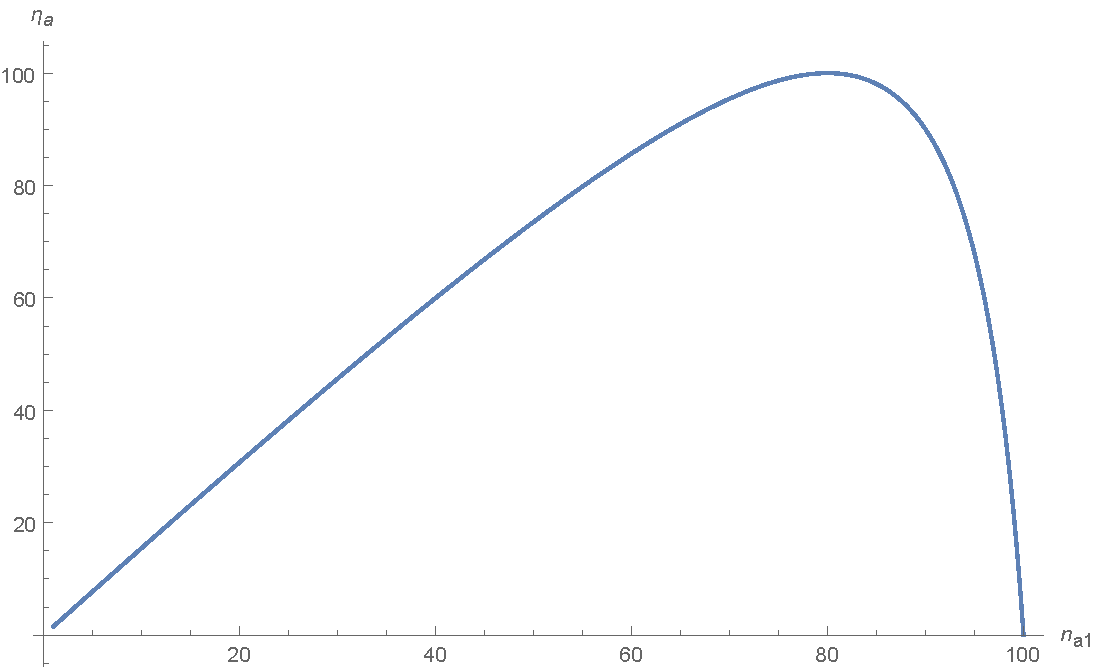
\includegraphics[width=.5\textwidth]{samplehalves}
\end{figure}

\subsection{Targeted Sampling}
Sample a equal number of points from each arm - until the error on all arms is smaller than some threshold. Then exploit. This should do better than observe-exploit, particularly where the probability of some events occurring without intervention is low.

A more sophisticated version:





\subsection{UCB variant}
Combine estimators according to:

\eq {
w_a     &= \frac{n_a}{\sum_{a=1}^K n_a} \text{ and } n_{i,j}=\begin{cases} 
n_{i,j} & \text{if } a = i \\
\frac{1}{2}\min\set{\frac{n_{a,1}}{p_a}, \frac{n_{a,0}}{1-p_a}}  & \text{otherwise}
\end{cases}
}

In this case the estimators from section \ref{sec:estimators} are biased - so its a lot harder to prove a regret bound. 

\begin{theorem} (Probably False) With probability at least $1 - \delta$ we have that:
$\displaystyle \left|\hat{\mu}_t - \mu\right| \leq \sqrt{\frac{\beta}{\sum_{a} n_a} \log{1 \over \delta}}$,
where $\beta > 0$ is some constant.
\end{theorem}

\begin{proof}
First note that $n_{a,b}$ is a random variable that is bounded by $t$ for all $a,b$.
We use the short-hand $\mu^{a,b}_{i,j} = \E[q(X) | X_i = j, X_a = b]$. Then
\eq{
\mu_{i,j} = p_a \mu_{i,j}^{a,1} + (1 - p_a) \mu_{i,j}^{a,0}\,.
}
Now we can apply Hoeffding's bound and the union bound to show that
\eq{
\P{\left|\frac{m_{a,b}}{n_{a,b}} - \mu_{i,j}^{a,b}\right| \geq \sqrt{\frac{1}{2n_{a,b}} \log \frac{4t}{\delta}}} \leq \frac{\delta}{2}\,.
}
Therefore by the union bound
\eq{
\P{\left|p_a \frac{m_{a,1}}{n_{a,1}} + (1 - p_a) \frac{m_{a,0}}{n_{a,0}} - \mu_{i,j}\right| \geq p_a \sqrt{\frac{1}{2n_{a,1}} \log\frac{4t}{\delta}}
+ (1 - p_a) \sqrt{\frac{1}{2n_{a,0}}\log\frac{4t}{\delta}}} \leq \delta\,
}
Now by Jensen's inequality 
\eq{
p_a \sqrt{\frac{1}{2n_{a,1}}\log\frac{4t}{\delta}} + (1 - p_a) \sqrt{\frac{1}{2n_{a,0}}\log\frac{4t}{\delta}}
&\leq \sqrt{\left(\frac{p_a}{2n_{a,1}} + \frac{1-p_a}{2n_{a,0}}\right)\log \frac{4t}{\delta}} \\
&\leq \sqrt{\max\set{\frac{p_a}{n_{a,1}}, \frac{1-p_a}{n_{a,0}}} \log\frac{4t}{\delta}} \\
&= \sqrt{{1 \over 2n_a} \log\frac{4t}{\delta}}\,.
}
Similarly,
\eq{
\P{\left|\frac{m_{i,j}}{n_{i,j}} - \mu_{i,j}\right| \geq \sqrt{\frac{1}{2n_a} \log\frac{4t}{\delta}}} \leq
\P{\left|\frac{m_{i,j}}{n_{i,j}} - \mu_{i,j}\right| \geq \sqrt{\frac{1}{2n_a} \log\frac{2t}{\delta}}} \leq \delta\,.
}
\end{proof}

\section{Algorithm}

\begin{algorithm}
\caption{UCB}
\begin{algorithmic}[1]
\State {\bf Input:} Number of variables $K$, vector $p \in [0,1]^K$, horizon $n$
\For{$t \in 1,\ldots,n$}
\For{$i \in 1,\ldots,K$}
\For{$j \in \set{0,1}$}
\State Compute $\tilde \mu_{i,j} = \hat \mu_{i,j} + \sqrt{\frac{\alpha}{\sum_{a} n_a} \log n}$ 
\EndFor
\EndFor
\State Choose $I_t, J_t = \argmax_{i,j} \tilde \mu_{i,j}$
\EndFor
\end{algorithmic}
\end{algorithm}

\section{Theorems}
\section{Experiments}



\begin{figure}[h]
\caption{Comparison of the performance of standard UCB versus causal UCB with $\beta=3$ and $\beta = 5$. 100 simulations were run for each algorithm up to a horizon of $10^5$ per value of $K$. Error bars span the 1st to 3rd quantile of the regret, round points mark the median and triangular points show the mean. For standard UCB the regret increases linearly with the number of arms $K$. For causal UCB the increase is sub-linear. Increasing $\beta$ leads to slower convergence but lower variance.}
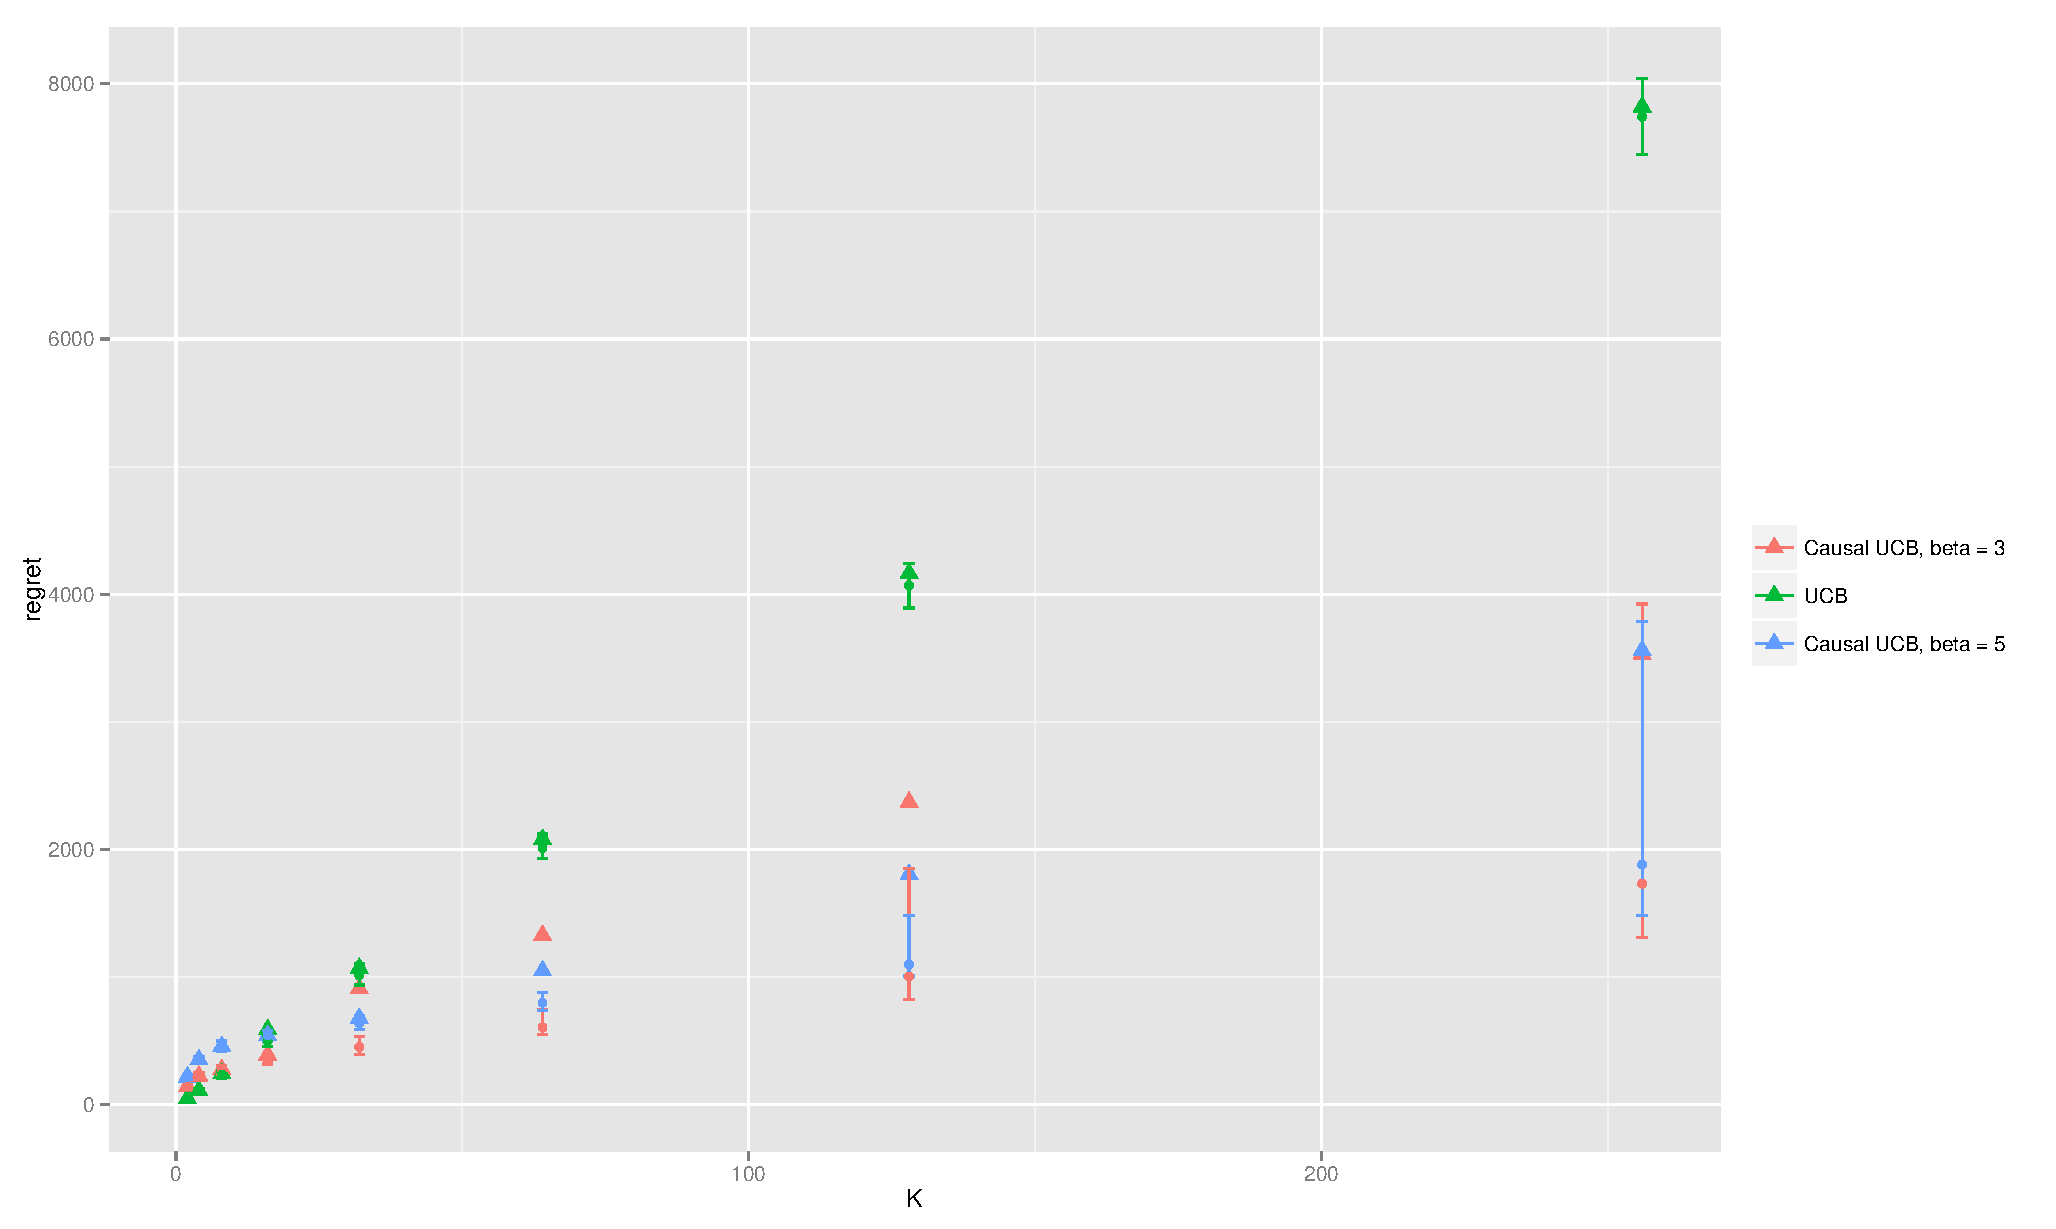
\includegraphics[width=1\textwidth]{regret_vs_K_series_beta.pdf}
\end{figure}

\begin{figure}[H]
\caption{The distribution of regret varies with the $\beta$ parameter in the bound in the estimator. As beta increases, the mean regret increases but the variance decreases. The plot shows the results of running $100$ independent bandits, with $K=256$ and $\epsilon=0.1$, up to a horizon $h=10^5$ for each value of $\beta$. }
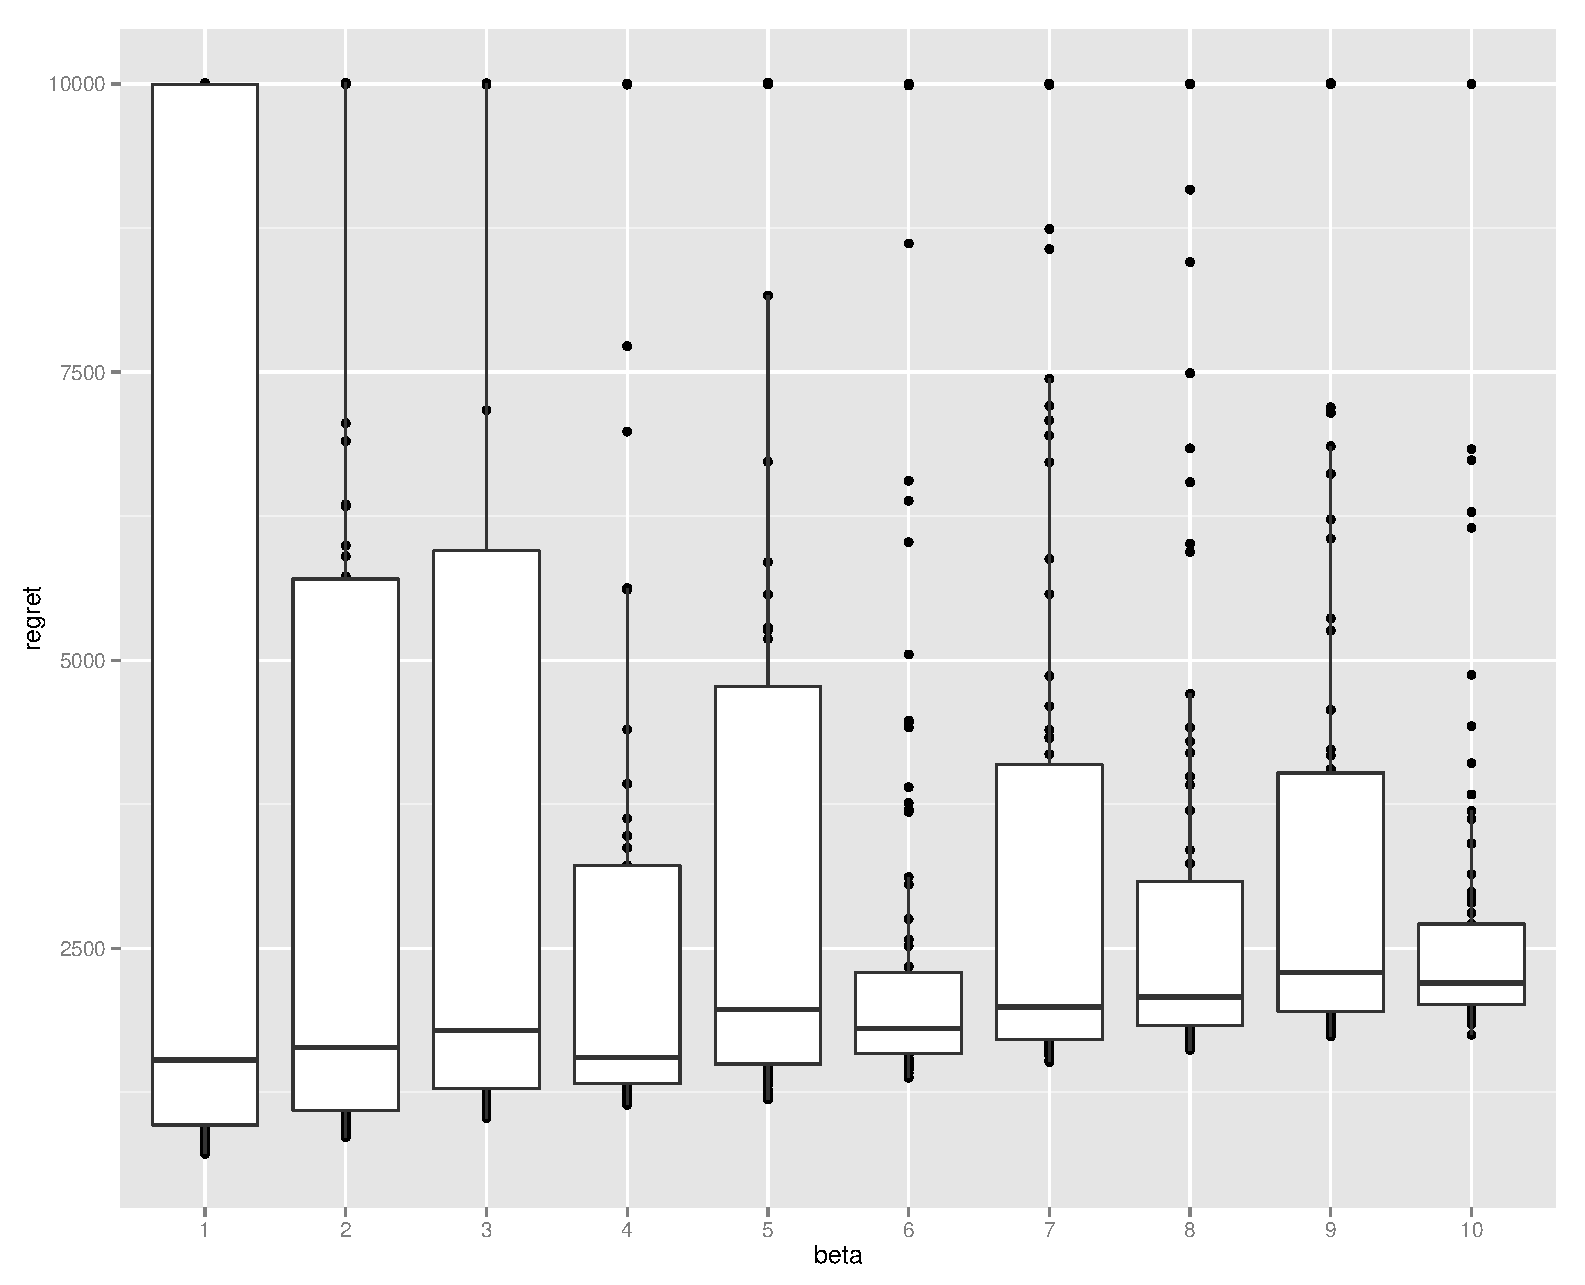
\includegraphics[width=0.7\textwidth]{regret_vs_beta_boxplot.pdf}
\end{figure}



Simululations to compare the performance of standard UCB with our modified algorithm. For each number of arms, $100$ bandits of each type were created and run upto to a horizon of $1000$ timesteps. The mean regret and its standard error from these simulations is plotted in figure \ref{fig:regretvsarms} The true data was generated from a model where:

\eq{
&p = [0.5]^{K}\\
&q(\boldsymbol{X}) = \begin{cases}0.5 & \text{if $X_{1}=0$}\\ 0.6 & \text{otherwise} \end{cases}
}






\section{Conclusion}

\newpage
\section{Notes}

\subsection{Why Hoeffdings bound doesn't hold if $n$ is a random variable}

Let $\{Z_1,Z_2...Z_n\} \sim Bernoulli(\frac{1}{2}) $ and $X_i = 2Z_i-1 \implies X_i \in \{-1,1\} \text{ and } E[X_i] = 0$.

For a fixed $n$, Hoeffdings inequality says: 
\eqn{
\label{eq:HoeffdingsRandom}
& P\left(|\frac{1}{n}\sum_{i=1}^{n}X_i| > \epsilon\right) \leq 2e^{-n\epsilon^2} \\
\implies & P \left(|\frac{1}{n}\sum_{i=1}^{n}X_i| > \sqrt{\frac{\log{4}}{n}}\right) \leq \frac{1}{2} \\
\implies & P\left( |\sum_{i=1}^{n}X_i| > \sqrt{n \log{4}}\right) \leq \frac{1}{2}
}


If $n$ is allowed to be dependent on the sequence of values sampled, this inequality no longer holds. 

\begin{proof}
Choose $n$ based on the sequence of samples seen so far such that:
\eq {
n = min \{ n: n > 4 \text{ and } \sum_{i=1}^{n}X_i > \sqrt{n \log \log n}\}
}
By the law of iterated logarithms this quantity is finite with probability $\sim 1$.

\eq {
& \implies  P\left( |\sum_{i=1}^{n}X_i| > \sqrt{n \log{\log{n}}}\right) \sim 1 \\
& \implies  P\left( |\sum_{i=1}^{n}X_i| > \sqrt{n \log{4}}\right) \sim 1 \text{, Since } \log{\log{n}} > \log{4} \;\; \forall n > 4 \\
}
 
Thus Hoeffdings inequality (equation \ref{eq:HoeffdingsRandom}) does not hold in general if $n$ is not independent of the samples $\{X_i\}$ (The bound does not work if you decide to stop sampling as soon as you reach a point where random walk fluctuations take you outside it)



\end{proof}


\bibliographystyle{plainnat}
\bibliography{c-bandit}

\end{document}


So the regret for the observe stage is bounded by:

\eqn {
R \leq \frac{2a}{\exp(a^2/(64+4a/3)) - 1}
}





But this is just the expected number of steps until one arm does not overlap. With more arms its more complicated - as we need the probability that $\alpha$ of them overlap (another union bound?).

\eqn {
E[n] = \sum_{t=1}^T P(n \geq t) \leq & \sum_{t=1}^\infty \left( \exp(-\frac{t\epsilon^2}{4+4\epsilon/3}) +exp(-\frac{t\epsilon^2}{4}) \right) \\
= & \frac{1}{\exp(\epsilon^2/(4+4\epsilon/3)) - 1} + \frac{1}{\exp(\epsilon^2/4) - 1} \\
\leq & \frac{2}{\exp(\epsilon^2/(4+4\epsilon/3)) - 1} \\
= & \frac{2}{\exp(a^2/(64+4a/3)) - 1}
}


\subsubsection{A very simple model}

So the regret for the observe stage is bounded by:

\eqn {
R \leq \frac{2a}{\exp(a^2/(64+4a/3)) - 1}
}





But this is just the expected number of steps until one arm does not overlap. With more arms its more complicated - as we need the probability that $\alpha$ of them overlap (another union bound?).
Lets try to analyse a very simple model in which the reward depends only on the value of $X_1$.

\eqn{
&P(Y|X_1=0,X_2,...X_N) = \frac{1}{2}-a\\
&P(Y|X_1=1,X_2,...X_N) = \frac{1}{2}+a\\
&P(X_i = j) = \frac{1}{2} \;\;\; \forall (i,j)\\
&\implies P(Y) = \frac{1}{2} \\
&\implies R_n = aE[n]
}

The goal is now to find $E[n]$ (which will be a function of $a$)

Lets start by considering how long on average we need to observe until the lower bound on the optimal arm is higher than the upper bound on a single other arm, $i$, (with expected reward $\frac{1}{2}$)

If the following three statements hold, then there is no overlap $LB^* = \hat{\mu}^* - \epsilon > UB_i = \hat{\mu}_i + \epsilon$.

\eqn {
\label{eq:overlap1}
&\mu^* - \hat{\mu}^* \leq \epsilon \\
\label{eq:overlap2}
&\hat{\mu}_i - \mu_i \leq \epsilon \\
\label{eq:overlap3}
&\epsilon \leq a/4
}

If \ref{eq:overlap3} is true, we can bound the probability of overlap  been the confidence intervals of the best arm and one of the other arms, $k$, at some timestep $t$ with the union bound of the probability that either \ref{eq:overlap1} or \ref{eq:overlap2} are false FOR ALL ARMS.

\eqn {
\rho(t) \equiv P(overlap_k) \leq 
P(\mu^* - \hat{\mu}^* \geq \epsilon) + P(\hat{\mu}_k - \mu_k \geq \epsilon)  \;\;\;\text{ if } \epsilon \leq a/4
}


Now the estimators and their bounds are independent, as they are composed from sums of independent variables $X_i$ so the probability that $\alpha$ of them have overlapping bounds is given by a binomial distribution. 

\eqn {
P(O > \alpha)  = & P(n \geq t) = 1 - \sum_{i=1}^\alpha \binom{K-1}{i}\rho(t)^{i}(1-\rho(t))^{K-1-i} \\
\leq & \exp(-(K-1)D(\frac{\alpha}{K-1} || \rho(t))
} 

 

\eqn {
P(|\hat{\mu}_{a0} -\mu_{a0}| > \epsilon_{a0}) \leq \delta/2 \;\; \text{ where } 
\epsilon_{a0}=\sqrt{\frac{1}{2n_{a0}}\log{\frac{4}{\delta}}}\\ 
P(|\hat{\mu}_{a1} -\mu_{a1}| > \epsilon_{a1}) \leq \delta/2 \;\; \text{ where } 
\epsilon_{a1}=\sqrt{\frac{1}{2n_{a1}}\log{\frac{4}{\delta}}}\\ 
}

We should not need $t$ in here since, although $n_{aj}$ is still random, its not dependent on previous results. 

Combining these two halves and applying the union bound gives:

\eqn{
P\left(|\hat{\mu}_a - \mu | > \sqrt{\frac{1}{2} \log{\frac{4}{\delta}}}
\left(p_a \sqrt{\frac{1}{2n_{a1}}}+(1-p_a) \sqrt{\frac{1}{2n_{a0}}} \right)\right) \leq \delta
}


I now need to pool these estimators for each $a \in \{1...K\}/I$ but I can't just use a union bound - I need the bound to shrink by combining the multiple estimates. 

For some distributions, 

